\documentclass{article}
\usepackage{graphicx} 
\usepackage{caption}  
\usepackage{hyperref}
\begin{document}

\title{GNU PLOTS}
\author{Rithika}
\date{\today}
\maketitle



\section*{1}
Figure~\ref{a}  

\begin{figure}[h!]
    \centering
    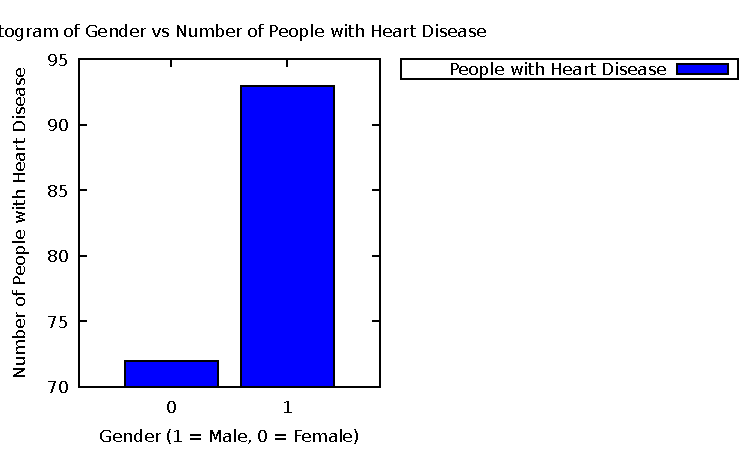
\includegraphics[width=0.6\textwidth]{4a.pdf}
    \caption{Histogram}
    \label{a}
\end{figure}


 Figure~\ref{b}  

\begin{figure}[h!]
    \centering
    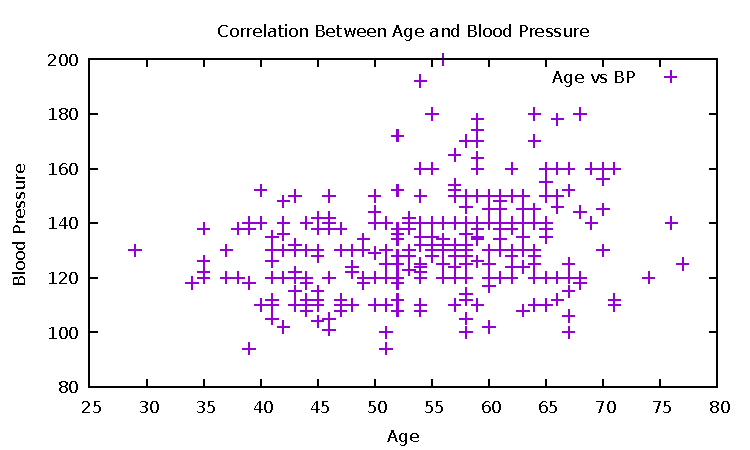
\includegraphics[width=0.6\textwidth]{4b.pdf}
    \caption{Points}
    \label{b}
\end{figure}

 Figure~\ref{c}  

\begin{figure}[h!]
    \centering
    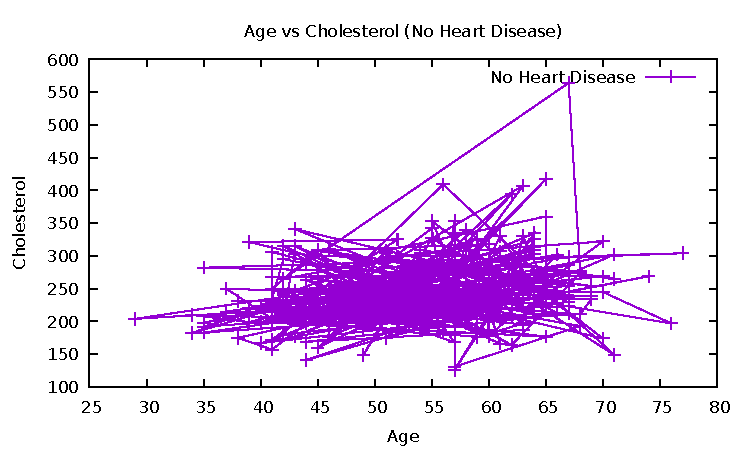
\includegraphics[width=0.6\textwidth]{4c.pdf}
    \caption{Linepoints}
    \label{c}
\end{figure}

 Figure~\ref{d}  

\begin{figure}[h!]
    \centering
    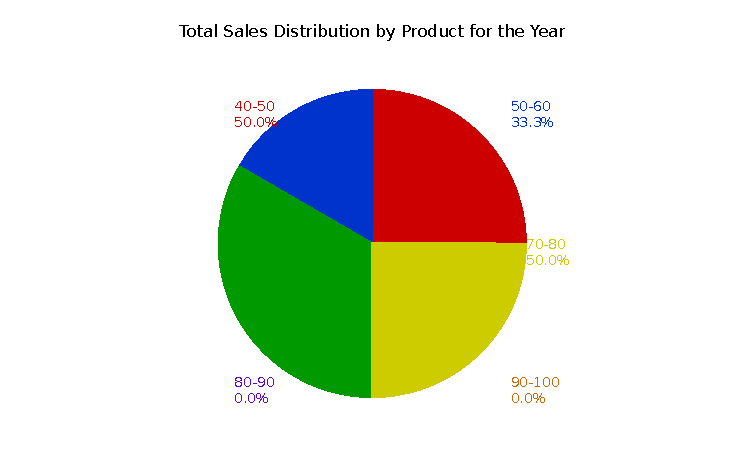
\includegraphics[width=0.6\textwidth]{d.pdf}
    \caption{Piechart}
    \label{d}
\end{figure}

\end{document}
